\chapter{Implementacija i korisničko sučelje}
		
		
		\section{Korištene tehnologije i alati}
		
			\textbf{\textit{dio 2. revizije}}
			
			 \textit{Detaljno navesti sve tehnologije i alate koji su primijenjeni pri izradi dokumentacije i aplikacije. Ukratko ih opisati, te navesti njihovo značenje i mjesto primjene. Za svaki navedeni alat i tehnologiju je potrebno \textbf{navesti internet poveznicu} gdje se mogu preuzeti ili više saznati o njima}.
			
			Pri izradi dokumentacije korišten je \textbf{LaTeX}\footnote{https://www.latex-project.org/} - markup jezik najčešće korišten za znanstvene publikacije. Za izradu dokumenta korišten je \textbf{TeXstudio}\footnote{https://www.texstudio.org/} - uređivač teksta prilagođen LaTeXu. Za izradu UML dijagrama u sklopu dokumentacije korišten je alat \textbf{Astah UML}\footnote{https://astah.net/products/astah-uml/}.
			
			Udaljeni repozitorij projekta dostupan je na web platformi \textbf{GitHub}\footnote{https://github.com/}. GitHub je korišten za pohranu izvornog koda i dokumentacije. 
			
			Kao razvojno okruženje korišten je \textbf{IntelliJ IDEA}\footnote{https://www.jetbrains.com/idea/}.
			
			Za izradu \textit{backenda} korišten je radni okvir \textbf{Spring Boot}\footnote{https://spring.io/projects/spring-boot/} i objektno orijentirani programski jezik \textbf{Java}\footnote{https://www.java.com/en/}. Spring Boot je specijalizacija radnog okvira Spring s ciljem jednostavnijeg i bržeg oblikovanja web aplikacije.
			
			Za izradu \textit{frontenda} korišten je \textbf{React}\footnote{https://react.dev/} i JavaScript ekstenzija \textbf{JavaScript XML}\footnote{https://legacy.reactjs.org/docs/introducing-jsx.html}. React, također poznat kao React.js ili ReactJS, je biblioteka u JavaScriptu za izgradnju korisničkih sučelja. Održavana je od strane Facebooka. React se najčešće koristi kao osnova u razvoju web ili mobilnih aplikacija. Složene aplikacije u Reactu obično zahtijevaju korištenje dodatnih biblioteka za interakciju s API-jem.
			
			Za izradu baze podataka korišten je sustav za upravljanje bazama podataka \textbf{PostgreSQL}\footnote{https://www.postgresql.org/}. Za pristup PostgreSQL sustavu baze podataka korišten je \textbf{pgAdmin 4}\footnote{https://www.pgadmin.org/} program. Za izradu E-R dijagraama baze podataka korišten je \textbf{ERDPlus}\footnote{https://erdplus.com/} alat.
			
			Komunikacija u timu realizirana je korištenjem aplikacija \textbf{WhatsApp}\footnote{https://www.whatsapp.com/} i \textbf{Discord}\footnote{https://discord.com/}.
			
			\eject 
		
	
		\section{Ispitivanje programskog rješenja}
			
			\textbf{\textit{dio 2. revizije}}\\
			
			 \textit{U ovom poglavlju je potrebno opisati provedbu ispitivanja implementiranih funkcionalnosti na razini komponenti i na razini cijelog sustava s prikazom odabranih ispitnih slučajeva. Studenti trebaju ispitati temeljnu funkcionalnost i rubne uvjete.}
	
			
			\subsection{Ispitivanje komponenti}
			\textit{Potrebno je provesti ispitivanje jedinica (engl. unit testing) nad razredima koji implementiraju temeljne funkcionalnosti. Razraditi \textbf{minimalno 6 ispitnih slučajeva} u kojima će se ispitati redovni slučajevi, rubni uvjeti te izazivanje pogreške (engl. exception throwing). Poželjno je stvoriti i ispitni slučaj koji koristi funkcionalnosti koje nisu implementirane. Potrebno je priložiti izvorni kôd svih ispitnih slučajeva te prikaz rezultata izvođenja ispita u razvojnom okruženju (prolaz/pad ispita). }
			
			
			
			\subsection{Ispitivanje sustava}
			
			 \textit{Potrebno je provesti i opisati ispitivanje sustava koristeći radni okvir Selenium\footnote{\url{https://www.seleniumhq.org/}}. Razraditi \textbf{minimalno 4 ispitna slučaja} u kojima će se ispitati redovni slučajevi, rubni uvjeti te poziv funkcionalnosti koja nije implementirana/izaziva pogrešku kako bi se vidjelo na koji način sustav reagira kada nešto nije u potpunosti ostvareno. Ispitni slučaj se treba sastojati od ulaza (npr. korisničko ime i lozinka), očekivanog izlaza ili rezultata, koraka ispitivanja i dobivenog izlaza ili rezultata.\\ }
			 
			 \textit{Izradu ispitnih slučajeva pomoću radnog okvira Selenium moguće je provesti pomoću jednog od sljedeća dva alata:}
			 \begin{itemize}
			 	\item \textit{dodatak za preglednik \textbf{Selenium IDE} - snimanje korisnikovih akcija radi automatskog ponavljanja ispita	}
			 	\item \textit{\textbf{Selenium WebDriver} - podrška za pisanje ispita u jezicima Java, C\#, PHP koristeći posebno programsko sučelje.}
			 \end{itemize}
		 	\textit{Detalji o korištenju alata Selenium bit će prikazani na posebnom predavanju tijekom semestra.}
			
			\eject 
		
		
		\section{Dijagram razmještaja}
			
			\textbf{\textit{dio 2. revizije}}
			
			 \textit{Potrebno je umetnuti \textbf{specifikacijski} dijagram razmještaja i opisati ga. Moguće je umjesto specifikacijskog dijagrama razmještaja umetnuti dijagram razmještaja instanci, pod uvjetom da taj dijagram bolje opisuje neki važniji dio sustava.}
			 
			 Dijagram razmještaja prikazuje odnos sklopovskih dijelova sustava međusobno i s programskim rješenjima koja su potrebna za korisnikovu interakciju s aplikacijom. Kao dio udaljene poslužiteljske infrastrukture postoje dva poslužiteljska računala: mrežni poslužitelj i poslužitelj baze podataka. Na mrežnom poslužitelju je aktivan proces programa aplikacije koji komunicira s bazom podataka koja je aktivna na vlastitom poslužitelju. Predviđeno je da korisnik koristi mrežni preglednik na vlastitom računalu za komunikaciju s aplikacijom na mrežnom poslužitelju.
			 
			 \begin{figure} [hbt!]
			 	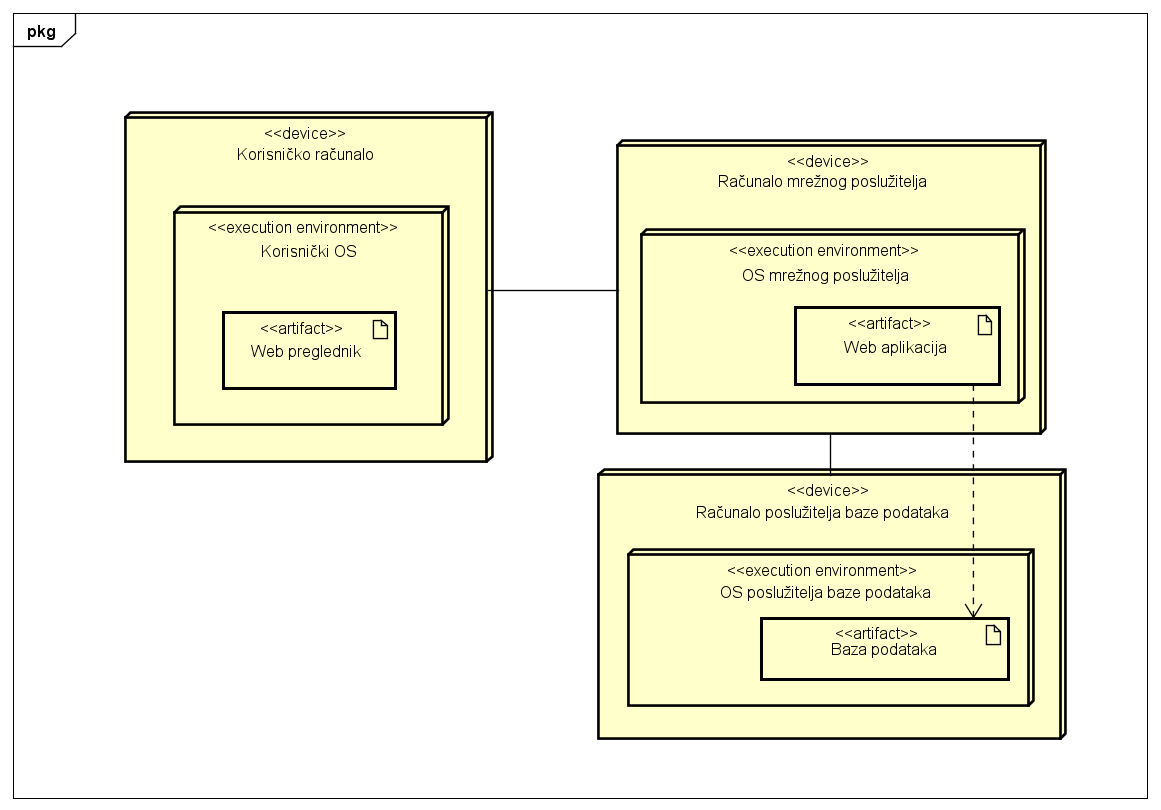
\includegraphics[width=\linewidth]{Slike/DeploymentDiagram}
			 	\caption{Dijagram razmještaja}
			 \end{figure}
			
			\eject 
		
		\section{Upute za puštanje u pogon}
		
			\textbf{\textit{dio 2. revizije}}\\
		
			 \textit{U ovom poglavlju potrebno je dati upute za puštanje u pogon (engl. deployment) ostvarene aplikacije. Na primjer, za web aplikacije, opisati postupak kojim se od izvornog kôda dolazi do potpuno postavljene baze podataka i poslužitelja koji odgovara na upite korisnika. Za mobilnu aplikaciju, postupak kojim se aplikacija izgradi, te postavi na neku od trgovina. Za stolnu (engl. desktop) aplikaciju, postupak kojim se aplikacija instalira na računalo. Ukoliko mobilne i stolne aplikacije komuniciraju s poslužiteljem i/ili bazom podataka, opisati i postupak njihovog postavljanja. Pri izradi uputa preporučuje se \textbf{naglasiti korake instalacije uporabom natuknica} te koristiti što je više moguće \textbf{slike ekrana} (engl. screenshots) kako bi upute bile jasne i jednostavne za slijediti.}
			
			
			 \textit{Dovršenu aplikaciju potrebno je pokrenuti na javno dostupnom poslužitelju. Studentima se preporuča korištenje neke od sljedećih besplatnih usluga: \href{https://aws.amazon.com/}{Amazon AWS}, \href{https://azure.microsoft.com/en-us/}{Microsoft Azure} ili \href{https://www.heroku.com/}{Heroku}. Mobilne aplikacije trebaju biti objavljene na F-Droid, Google Play ili Amazon App trgovini.}
			
			
			\eject 